%\documentclass{beamer}
%\usetheme{Pittsburgh} 
\documentclass{scrartcl}

\usepackage[utf8]{inputenc}
\usepackage{default}
\usepackage[procnames]{listings}
\usepackage{graphicx}
%\usepackage[toc,page]{appendix}
\usepackage{caption}
\usepackage{hyperref}
\usepackage{color}
\usepackage[T1]{fontenc}

%Python
\definecolor{keywords}{RGB}{255,0,90}
\definecolor{comments}{RGB}{0,0,113}
\definecolor{red}{RGB}{160,0,0}
\definecolor{green}{RGB}{0,150,0}
\lstset{language=Python,
basicstyle=\ttfamily\scriptsize,
keywordstyle=\color{keywords},
commentstyle=\color{comments},
stringstyle=\color{red},
identifierstyle=\color{green},
procnamekeys={def,class},
breaklines=true,
columns=fullflexible,
%Numbering and Tabs
%numbers=left,
%tabsize=4,
%showspaces=false,
%showstringspaces=false
}


%Bibliogrpahy?
%\usepackage{bibentry}
%\nobibliography*
%\bibentry{ }


\begin{document}

\title{Evolutionary Computation Theory and Application}
\subtitle{Report}
\author{
  Quignon, Christophe \\
  \href{https://github.com/ChrisQuignon/ECTA}{github.com/ChrisQuignon/ECTA}
  %Familyname, Name
} 
\date{\today}


\maketitle


\setcounter{tocdepth}{2}
\setcounter{secnumdepth}{2}
\tableofcontents{}


\section{Optimization}
%Theoretic description

\subsection{Problem}
\subsubsection{Square error}
\subsubsection{Trimodal fitness function}
\subsubsection{3D Plateau fitness function}
%characteristics of the problem

\subsection{Algorithms}
\subsubsection{Basic Steepest Descent}
\subsubsection{Steepest Descent with momentum}
\subsubsection{Newton’s Method}
%How do we solve it

\subsection{Parameters}
%What could be changed
\subsubsection{Starting Positions}
\subsubsection{Learning Rates}
\subsubsection{Momentum}

\subsection{Analysis}
%what happened and why

\subsubsection{Fitness}

%MEANMAX
\begin{figure}[H]
\centering
\begin{minipage}{.5\textwidth}
  \centering
  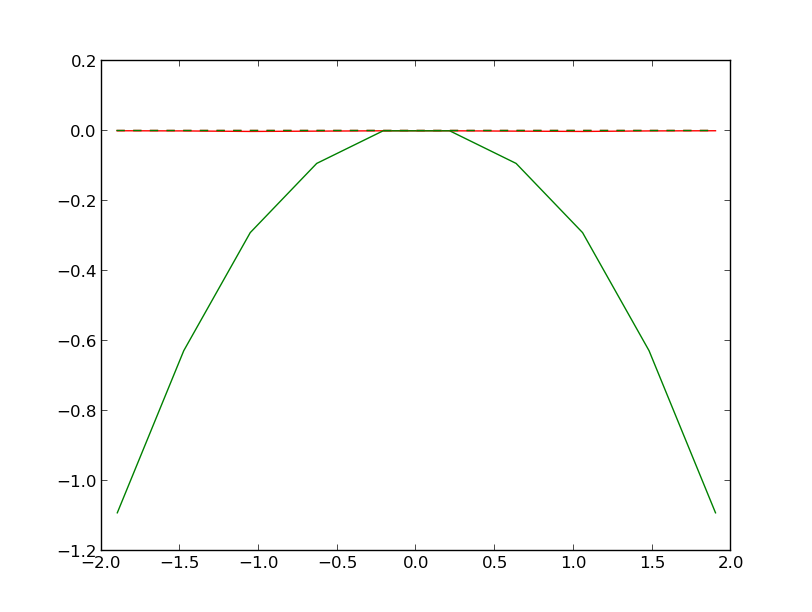
\includegraphics[width=.8\linewidth]{img/ex1/analysis_squared_newton_hill.png}
  %\caption{}
  %\label{fig:}
\end{minipage}%
\begin{minipage}{.5\textwidth}
  \centering
  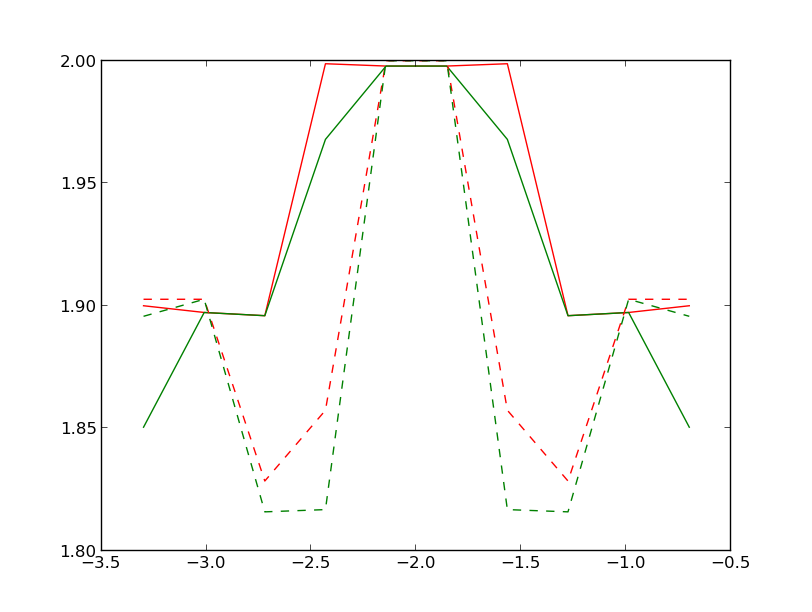
\includegraphics[width=.8\linewidth]{img/ex1/analysis_trimodal_newton_hill.png}
  %\caption{}
  %\label{fig:} 
\end{minipage}
\caption{Fitness analysis of the mean (green) and maximal(red) values of the newton method (dotted) and the Hillclimber (solid).}
\label{fig:}
\end{figure}
%Description

%HEATMAPS
\begin{figure}[H]
\centering
\begin{minipage}{.5\textwidth}
  \centering
  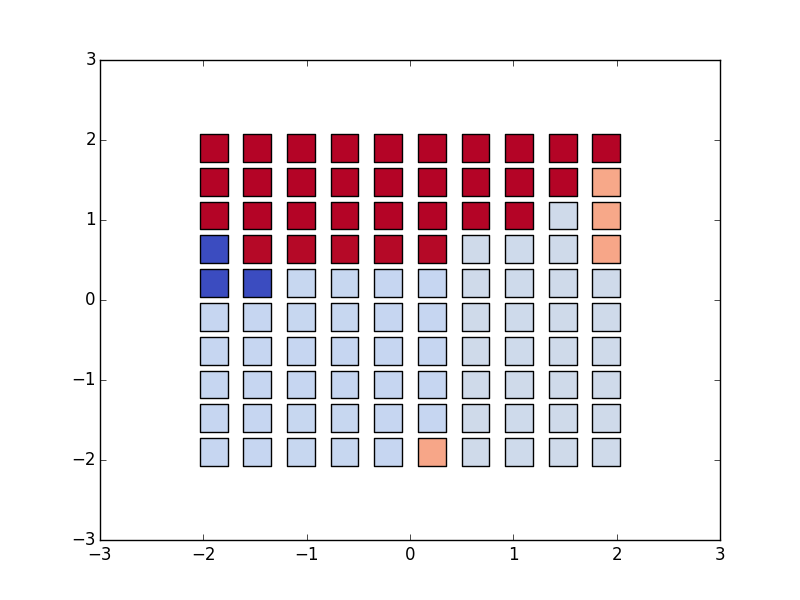
\includegraphics[width=.8\linewidth]{img/ex1/Heatmap_HC.png}
  %\caption{}
  %\label{fig:}
\end{minipage}%
\begin{minipage}{.5\textwidth}
  \centering
  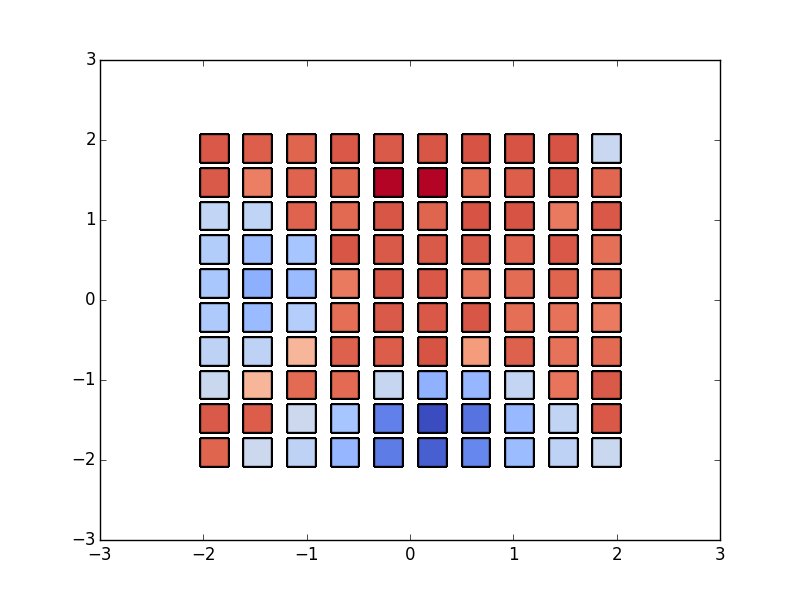
\includegraphics[width=.8\linewidth]{img/ex1/Heatmap_SS.png}
  %\caption{}
  %\label{fig:} 
\end{minipage}
\caption{Heatmap of the fitness values of the Hillclimber (left) and Steepest Descent(right) method in a 3D Landscape.}
\label{fig:}
\end{figure}

%INERTIA LEARNING
\begin{figure}[H]
\centering
\begin{minipage}{.5\textwidth}
  \centering
  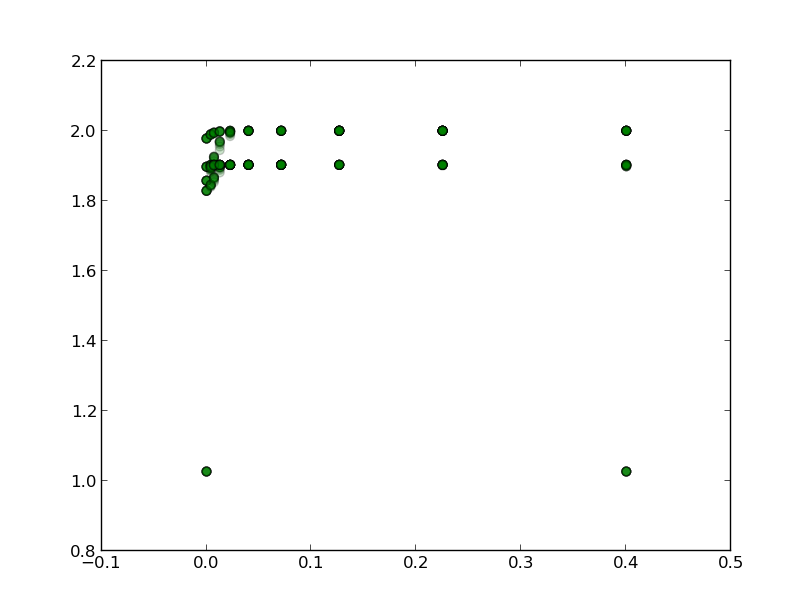
\includegraphics[width=.8\linewidth]{img/ex1/learning_trimodal_ss.png}
  %\caption{}
  %\label{fig:}
\end{minipage}%
\begin{minipage}{.5\textwidth}
  \centering
  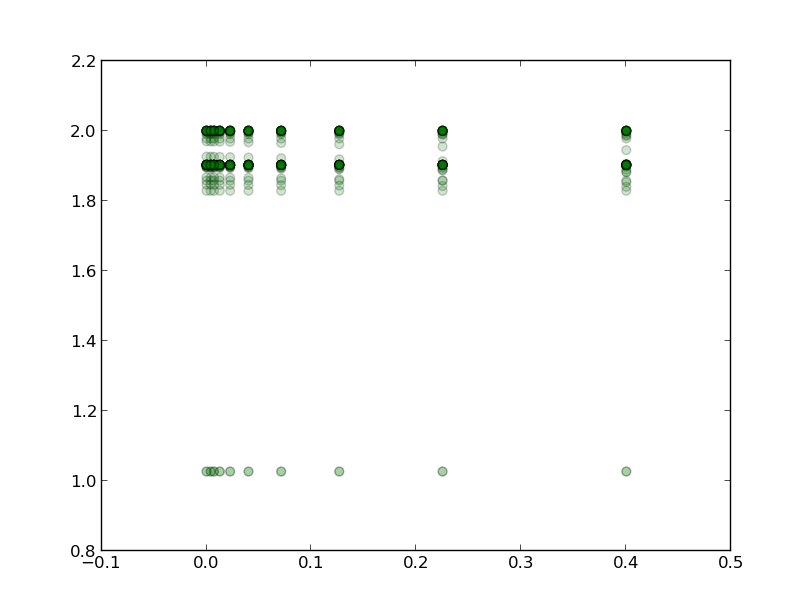
\includegraphics[width=.8\linewidth]{img/ex1/inertia_trimodal_ss.png}
  %\caption{}
  %\label{fig:} 
\end{minipage}
\caption{Comparison of the fitness values with respect to the learning rate (left) and inertia(right) with the steepest descent method on the trimodal landscape.}
\label{fig:}
\end{figure}

\subsubsection{Best result}

%PLATEAU
\begin{figure}[H]
\centering
\begin{minipage}{.5\textwidth}
  \centering
  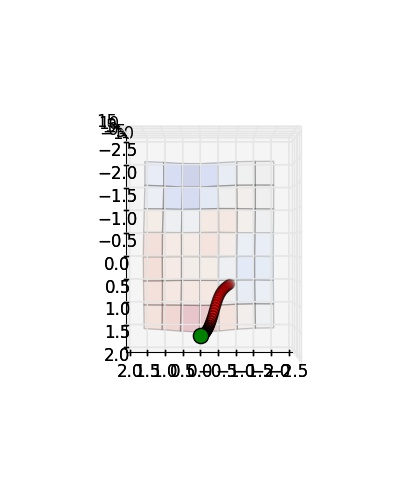
\includegraphics[width=.8\linewidth]{img/ex1/runs/SD-Plateau3D_0_0,07.jpg}
  %was SD-Plateau3D_-0.81  0.59_0.0_0.07
  %\caption{}
  %\label{fig:}
\end{minipage}%
\begin{minipage}{.5\textwidth}
  \centering
  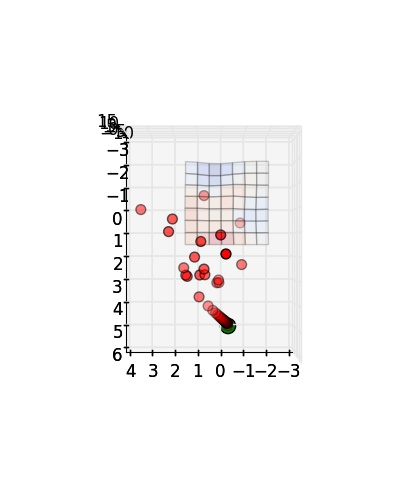
\includegraphics[width=.8\linewidth]{img/ex1/runs/SD-Plateau3D_0,22_0,02.jpg}
  %\caption{}
  %\label{fig:} 
\end{minipage}
\caption{Two highly different runs of the steepest descent algorithm in the Plateau3D landscape. Learning rates of 0.0 (left) and 0.22 (right) and inertia 0.07 (left) and 0.02 (right).}
\label{fig:}
\end{figure}


%RUNS
\begin{figure}[H]
\centering
\begin{minipage}{.5\textwidth}
  \centering
  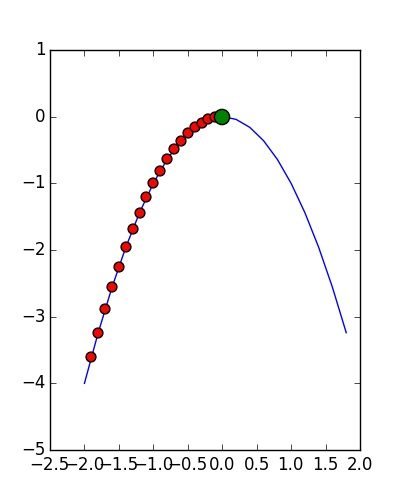
\includegraphics[width=.8\linewidth]{img/ex1/runs/HC-SquaredError2D_-1,9.jpg}
  %\caption{}
  %\label{fig:}
\end{minipage}%
\begin{minipage}{.5\textwidth}
  \centering
  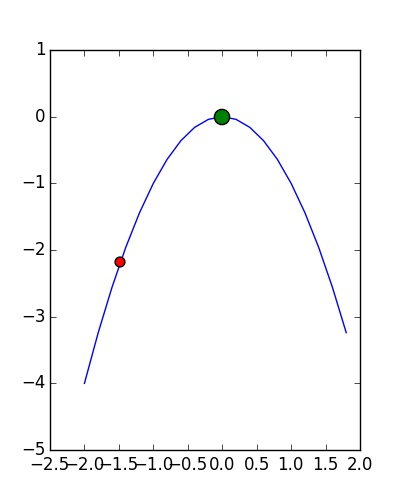
\includegraphics[width=.8\linewidth]{img/ex1/runs/NM-SquaredError2D_-1,48.jpg}
  %\caption{}
  %\label{fig:} 
\end{minipage}
\caption{Incrementing steps of optimization of the Hillclimber (left) and the Newton Method (right) on the squared error landscape.}
\label{fig:}
\end{figure}


\subsection{Conclusion}



\section{Genetic Algorithms}
%Theoretic description

\subsection{Problem}
%characteristics of the problem

\subsection{Algorithms}
%How do we solve it
real valued, bit string

\subsection{Parameters}
%What could be changed
\subsubsection{Population size}
\subsubsection{Selection}
\subsubsection{Crossover}
\subsubsection{Mutation}


\subsection{Analysis}
%what happened and why

\subsubsection{Parameter variations}

\subsubsection{Fitness}

\subsubsection{Best result}

\subsection{Conclusion}



\section{Travelling Salesman}
%Theoretic description

\subsection{Problem}
%characteristics of the problem
TSP

\subsection{Algorithms}
%How do we solve it

\subsubsection{Representation}
\paragraph{Priority list}
\paragraph{Permutations}

\subsection{Parameters}
%What could be changed
\subsubsection{Population size}

%TSP POP
\begin{figure}
 \center
 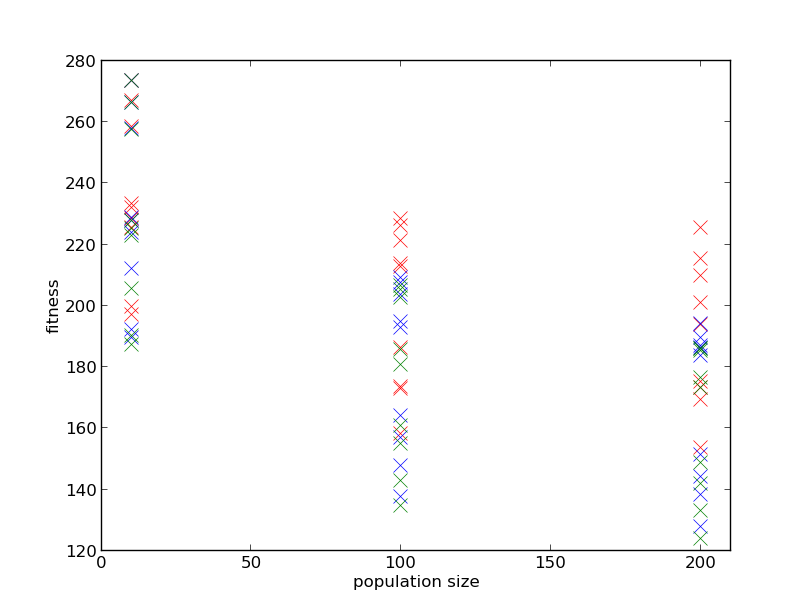
\includegraphics[width=.5\linewidth]{img/ex3/tsp_fitness_population.png}
 \caption{All fitness values (min=green, mean = blue, max = red))ordered by population.}
\end{figure}

\subsubsection{Selection Pressure} 

%TSP Selection
\begin{figure}
 \center
 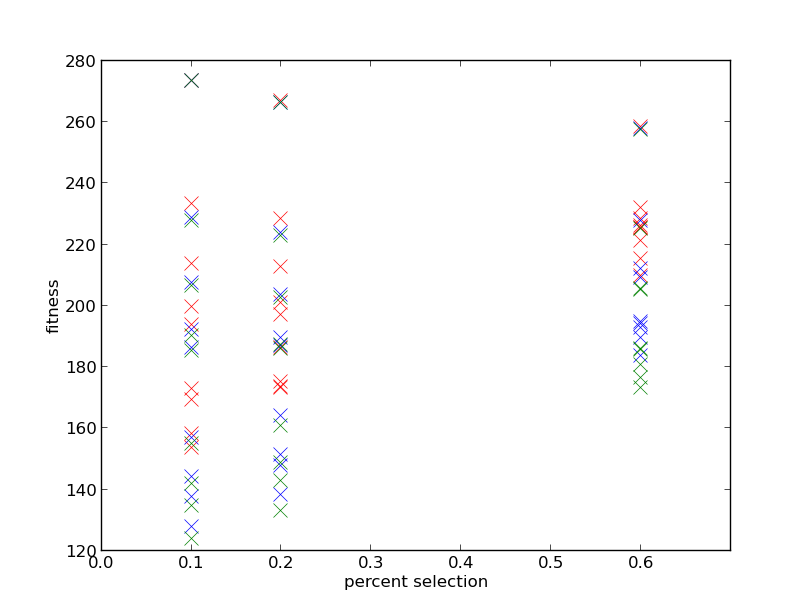
\includegraphics[width=.5\linewidth]{img/ex3/tsp_fitness_selection.png}
 \caption{All fitness values (min=green, mean = blue, max = red))ordered by selection pressure.}
\end{figure}


\subsubsection{Mutation}
%TSP mutations
\begin{figure}
 \center
 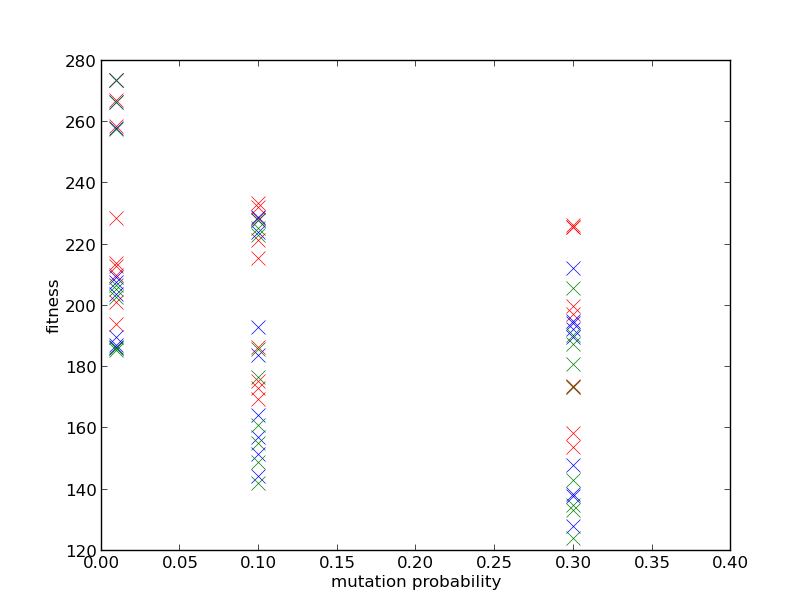
\includegraphics[width=.5\linewidth]{img/ex3/tsp_fitness_mutation.png}
 \caption{All fitness values (min=green, mean = blue, max = red))ordered by selection mutation.}
\end{figure}

\subsection{Analysis}
%what happened and why
Schema Theory
Building Block Hypothesis
Solution Validation

\subsubsection{Fitness}

\subsubsection{Best result}

%TSP BEST
\begin{figure}[H]
\centering
\begin{minipage}{.5\textwidth}
  \centering
  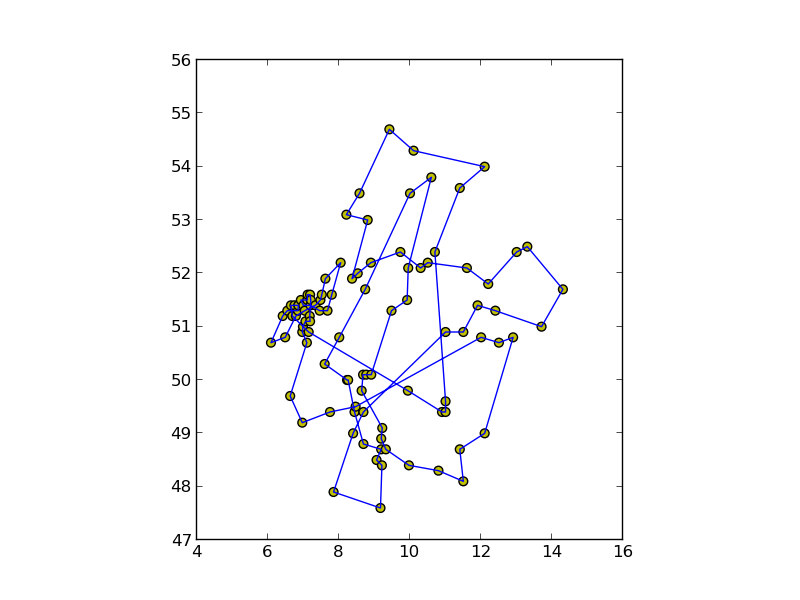
\includegraphics[width=.8\linewidth]{img/ex3/68,46-1-1000-200-0,2-0,6.png}
  %\caption{}
  %\label{fig:}
\end{minipage}%
\begin{minipage}{.5\textwidth}
  \centering
  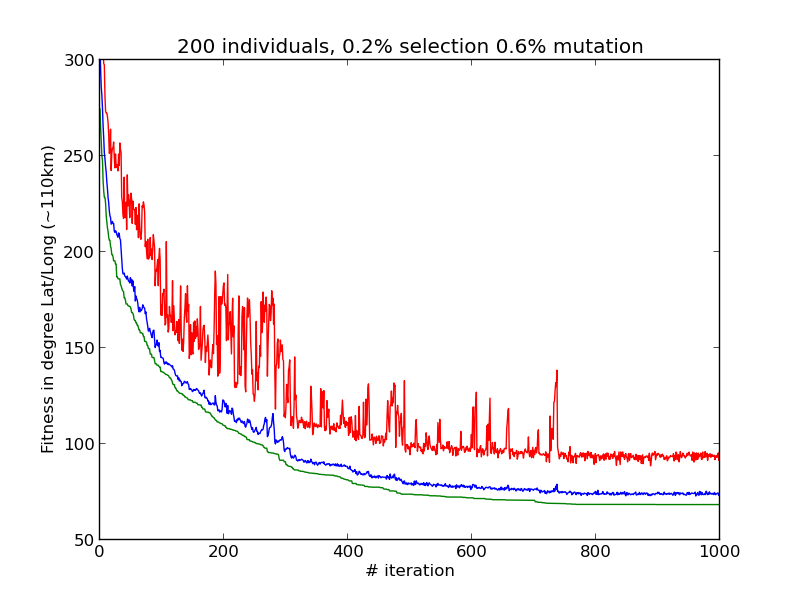
\includegraphics[width=.8\linewidth]{img/ex3/68,46-1-1000-200-0,2-0,6-fitness.png}
  %\caption{}
  %\label{fig:} 
\end{minipage}
\caption{The best run for the travelling salesman. 1k iterations with 200 individuals, a selection of 20\% and mutation rate of 60\% (not 0.2 and 0.6 as in the image). The position of the cities are given in Lat/Long, as well as the fitness. The fitness is given as max(red), mean(blue) and min(green).}
\label{fig:}
\end{figure}
%Description

\subsection{Conclusion}




\section{Evolutionary Algorithm}
%Theoretic description

\subsection{Problem}
%characteristics of the problem

\subsection{Algorithms}
%How do we solve it


\subsection{Parameters}
%What could be changed
\subsubsection{Iterations}
\subsubsection{Sigma/ Sigma Delta}

%SIGMA
\begin{figure}
 \center
 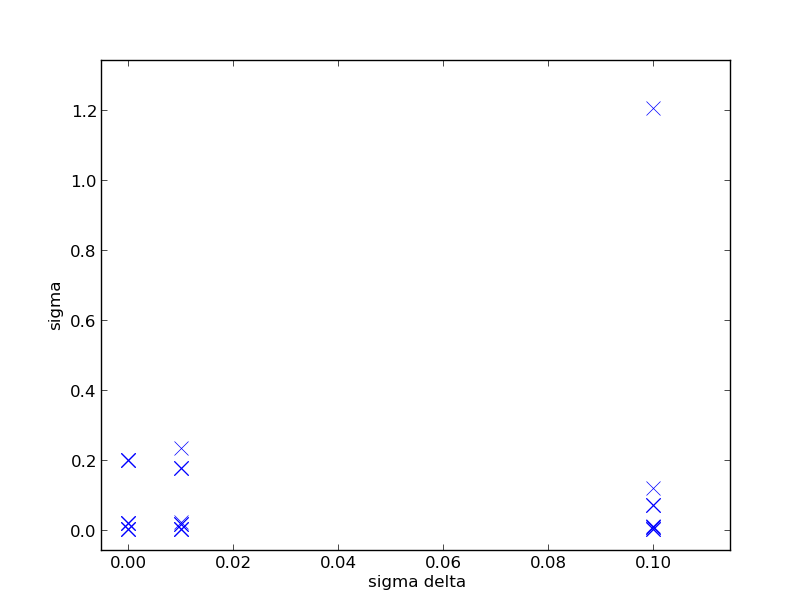
\includegraphics[width=.5\linewidth]{img/ex4/sigmas.png}
 \caption{Final sigma in relation to the sigma delta over all runs.}
\end{figure}

\subsubsection{selection Mode}
\paragraph{$1+1$}

\paragraph{$\mu,\lambda$}

\paragraph{$\mu +\lambda$}


\subsection{Analysis}
%what happened and why


\begin{table}[htbp]
\caption{Fitness over 30 runs each}
\begin{tabular}{r r r|r r }

selection & Sigma $\Delta$ & Sigma & Mean Fitness & Best Fitness \\ \hline
1+1 & 0 & 0.002 & 1228892 & 1228892 \\ 
1+1 & 0.01 & 0.002 & 1228793 & 1228561 \\ 
1+1 & 0.1 & 0.012 & 1225754 & 1221046 \\ 
1+1 & 0 & 0.02 & 1228892 & 1228892 \\ 
1+1 & 0.01 & 0.023 & 1228892 & 1228892 \\ 
1+1 & 0.1 & 0.121 & 1228892 & 1228892 \\ 
1+1 & 0 & 0.2 & 1228892 & 1228892 \\ 
1+1 & 0.01 & 0.234 & 1228892 & 1228892 \\ 
1+1 & 0.1 & 1.206 & 1228892 & 1228892 \\ 
1+20 & 0 & 0.002 & 1224793 & 1220197 \\ 
1+20 & 0.01 & 0.002 & 1220713 & 1213483 \\ 
1+20 & 0.1 & 0.001 & 1225500 & 1222800 \\ 
1+20 & 0 & 0.02 & 1227115 & 1226354 \\ 
1+20 & 0.01 & 0.018 & 1228892 & 1228892 \\ 
1+20 & 0.1 & 0.007 & 1225472 & 1221001 \\ 
1+20 & 0 & 0.2 & \textbf{1188537} & \textbf{1128005} \\ 
1+20 & 0.01 & 0.175 & 1228892 & 1228892 \\ 
1+20 & 0.1 & 0.07 & 1226681 & 1220602 \\ 
2+20 & 0 & 0.002 & 1225606 & 1223490 \\ 
2+20 & 0.01 & 0.002 & 1224471 & 1220651 \\ 
2+20 & 0.1 & 0.001 & 1226304 & 1224964 \\ 
2+20 & 0 & 0.02 & 1228892 & 1228892 \\ 
2+20 & 0.01 & 0.018 & 1227215 & 1221702 \\ 
2+20 & 0.1 & 0.007 & 1211559 & \textbf{1197249} \\ 
2+20 & 0 & 0.2 & 1218575 & \textbf{1190204} \\ 
2+20 & 0.01 & 0.175 & 1228892 & 1228892 \\ 
2+20 & 0.1 & 0.07 & 1228892 & 1228892 \\ 
1,20 & 0 & 0.002 & inf & inf \\ 
\dots & & & \dots & \dots \\
%1,20 & 0.01 & 0.002 & inf & inf \\ 
%1,20 & 0.1 & 0.002 & inf & inf \\ 
%1,20 & 0 & 0.02 & inf & inf \\ 
%1,20 & 0.01 & 0.018 & inf & inf \\ 
%1,20 & 0.1 & 0.007 & inf & inf \\ 
%1,20 & 0 & 0.2 & inf & inf \\ 
%1,20 & 0.01 & 0.175 & inf & inf \\ 
%1,20 & 0.1 & 0.07 & inf & inf \\ 
%2,20 & 0 & 0.002 & inf & inf \\ 
%2,2 & 0.01 & 0.002 & inf & inf \\ 
%2,20 & 0.1 & 0.002 & inf & inf \\ 
%2,20 & 0 & 0.02 & inf & inf \\ 
%2,20 & 0.01 & 0.018 & inf & inf \\ 
%2,20 & 0.1 & 0.007 & inf & inf \\ 
%2,20 & 0 & 0.2 & inf & inf \\ 
%2,20 & 0.01 & 0.175 & inf & inf \\ 
2,20 & 0.1 & 0.07 & inf & inf \\ 
\end{tabular}
\label{}
\end{table}


\subsubsection{Fitness}

\subsubsection{Best result}

%VEHICLE BEST
\begin{figure}
 \center
 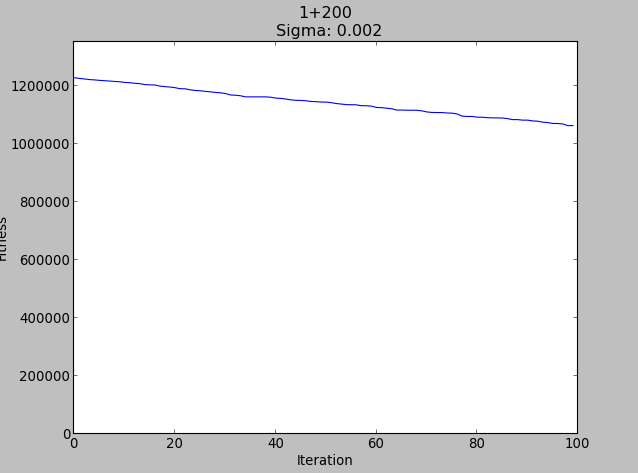
\includegraphics[width=.5\linewidth]{img/ex4/1063459-1+200-0,002.png}
 \caption{Screenshot of the best run with a final fitness of 1063459, and a fixed sigma of 0.002.}
\end{figure}


\subsection{Conclusion}


%CONTENTS
%NOTES


%COPY AND PASTE FROM HERE

%\begin{enumerate}
% \item 
%\end{enumerate}

%\hyperref{link}{text}

%\begin{lstlisting}[language=Python]
%#PYTHON CODE HERE
%\end{lstlisting}

%\lstinputlisting[Language=Python]{ }


%\begin{figure}
% \center
% \includegraphics[width= cm]{ }
% \caption{}
%\end{figure}


%\begin{figure}[H]
%\centering
%\begin{minipage}{.5\textwidth}
%  \centering
%  \includegraphics[width=.8\linewidth]{img/}
%  %\caption{}
%  %\label{fig:}
%\end{minipage}%
%\begin{minipage}{.5\textwidth}
%  \centering
%  \includegraphics[width=.8\linewidth]{img/}
%  %\caption{}
%  %\label{fig:} 
%\end{minipage}
%\caption{}
%\label{fig:}
%\end{figure}
%Description


%BIBLIOGRPAHY?
\bibliographystyle{plain}%amsalpha
\bibliography{Top30.bib}
%\bibentry{}

\end{document}
